% Created by tikzDevice version 0.12.3.1 on 2021-10-29 14:28:23
% !TEX encoding = UTF-8 Unicode
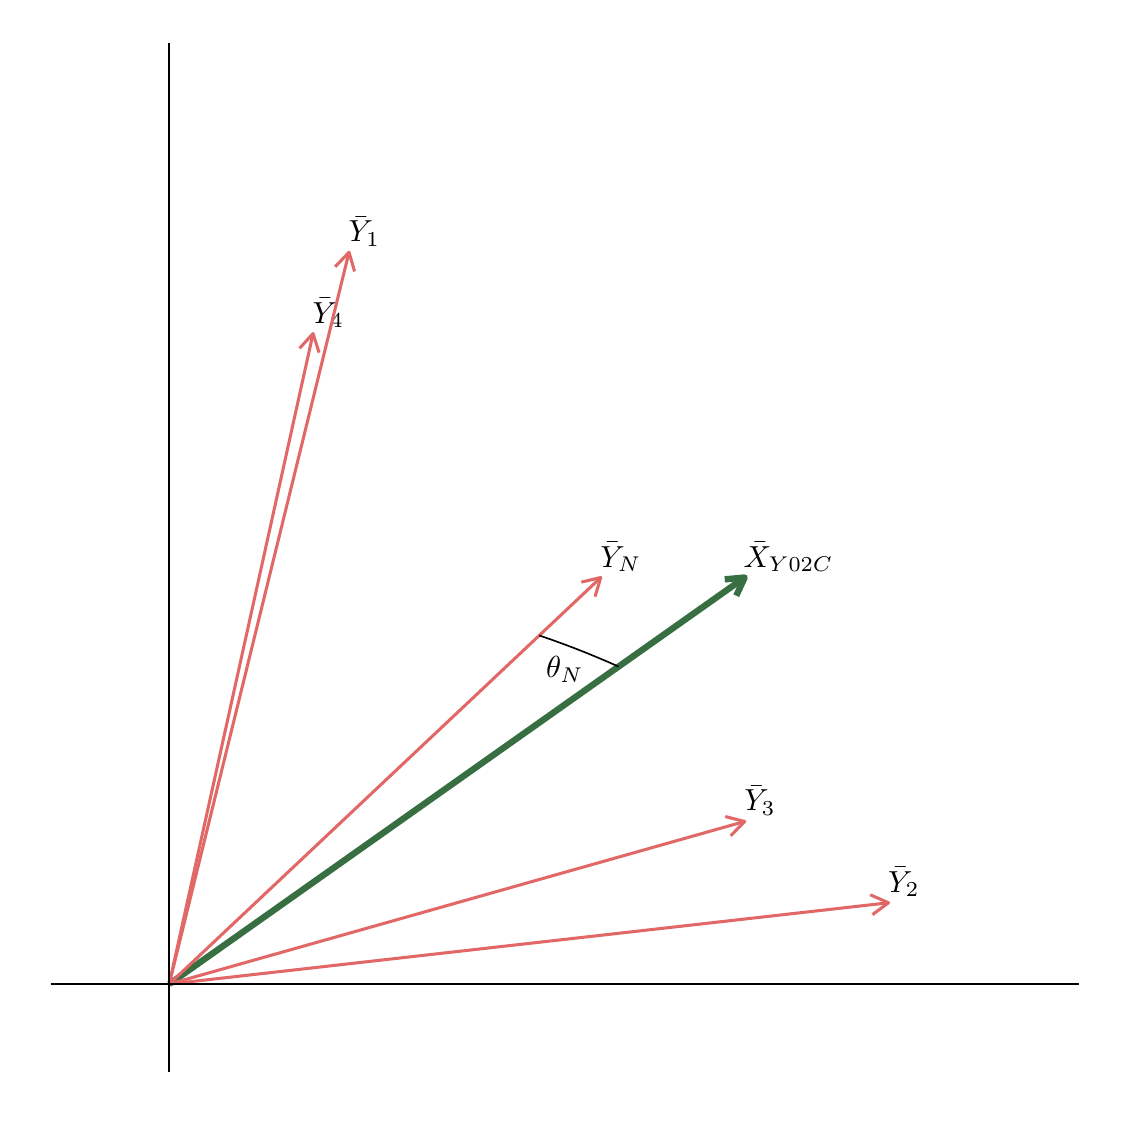
\begin{tikzpicture}[x=1pt,y=1pt]
\definecolor{fillColor}{RGB}{255,255,255}
\path[use as bounding box,fill=fillColor,fill opacity=0.00] (0,0) rectangle (385.44,385.44);
\begin{scope}
\path[clip] (  0.00,  0.00) rectangle (385.44,385.44);
\definecolor{drawColor}{RGB}{255,255,255}
\definecolor{fillColor}{RGB}{255,255,255}

\path[draw=drawColor,line width= 0.6pt,line join=round,line cap=round,fill=fillColor] (  0.00,  0.00) rectangle (385.44,385.44);
\end{scope}
\begin{scope}
\path[clip] (  8.25,  8.25) rectangle (379.94,379.94);
\definecolor{drawColor}{RGB}{0,0,0}

\node[text=drawColor,anchor=base west,inner sep=0pt, outer sep=0pt, scale=  1.10] at (258.75,190.55) {$\bar{X}_{Y02C}$};

\node[text=drawColor,anchor=base west,inner sep=0pt, outer sep=0pt, scale=  1.10] at (116.00,308.08) {$\bar{Y}_1$};

\node[text=drawColor,anchor=base west,inner sep=0pt, outer sep=0pt, scale=  1.10] at (310.95, 73.02) {$\bar{Y}_2$};

\node[text=drawColor,anchor=base west,inner sep=0pt, outer sep=0pt, scale=  1.10] at (258.96,102.40) {$\bar{Y}_3$};

\node[text=drawColor,anchor=base west,inner sep=0pt, outer sep=0pt, scale=  1.10] at (103.01,278.70) {$\bar{Y}_4$};

\node[text=drawColor,anchor=base west,inner sep=0pt, outer sep=0pt, scale=  1.10] at (206.94,190.55) {$\bar{Y}_N$};
\definecolor{drawColor}{RGB}{55,111,66}

\path[draw=drawColor,line width= 2.3pt,line join=round] ( 51.14, 39.84) -- (259.08,186.75);

\path[draw=drawColor,line width= 2.3pt,line join=round] (256.05,180.19) --
	(259.08,186.75) --
	(251.88,186.09);
\definecolor{drawColor}{RGB}{226,104,104}

\path[draw=drawColor,line width= 1.1pt,line join=round] ( 51.14, 39.84) -- (116.12,304.28);

\path[draw=drawColor,line width= 1.1pt,line join=round] (118.13,297.34) --
	(116.12,304.28) --
	(111.12,299.06);

\path[draw=drawColor,line width= 1.1pt,line join=round] ( 51.14, 39.84) -- (311.06, 69.22);

\path[draw=drawColor,line width= 1.1pt,line join=round] (305.25, 64.93) --
	(311.06, 69.22) --
	(304.44, 72.11);

\path[draw=drawColor,line width= 1.1pt,line join=round] ( 51.14, 39.84) -- (259.08, 98.60);

\path[draw=drawColor,line width= 1.1pt,line join=round] (254.04, 93.42) --
	(259.08, 98.60) --
	(252.07,100.38);

\path[draw=drawColor,line width= 1.1pt,line join=round] ( 51.14, 39.84) -- (103.12,274.90);

\path[draw=drawColor,line width= 1.1pt,line join=round] (105.30,268.01) --
	(103.12,274.90) --
	( 98.24,269.57);

\path[draw=drawColor,line width= 1.1pt,line join=round] ( 51.14, 39.84) -- (207.09,186.75);

\path[draw=drawColor,line width= 1.1pt,line join=round] (205.01,179.83) --
	(207.09,186.75) --
	(200.06,185.09);
\definecolor{drawColor}{RGB}{0,0,0}

\path[draw=drawColor,line width= 0.6pt,line join=round] (213.51,154.56) --
	(209.59,156.30) --
	(205.60,157.99) --
	(201.56,159.65) --
	(197.47,161.26) --
	(193.32,162.82) --
	(189.12,164.34) --
	(184.87,165.81);

\path[draw=drawColor,line width= 0.6pt,line join=round] (  8.25, 39.84) -- (379.94, 39.84);

\path[draw=drawColor,line width= 0.6pt,line join=round] ( 51.14,  8.25) -- ( 51.14,379.94);

\node[text=drawColor,anchor=base,inner sep=0pt, outer sep=0pt, scale=  1.10] at (194.10,150.63) {$\theta_N$};
\end{scope}
\end{tikzpicture}
